%%%%%%%%%%%%%%%%%%%%%%%%%%%%%%%%%%%%%%%%%%%%%%%%%%%%%section 2
\section{Learning to Answer Yes/No} % (fold)
\noindent
{\color{LightRubineRed} \rule{\linewidth}{1mm} }
\subsection{Perceptron}
\begin{align*}
h(x) &= sign((\sum_{i=1} W_i x_i - \text{threshold})) \\
     &= sign((\sum_{i=0} W_i x_i)) \\
     &= sign(W^TX)
\end{align*}
\begin{center}
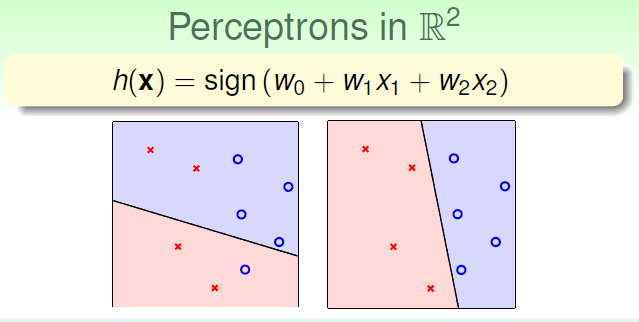
\includegraphics[width=10cm, height=5cm]{lecture2_1}\\
\end{center}
\begin{algorithm}  
\caption{Perceptron Learning Algorithm}  
\begin{algorithmic}  
\FOR{$t\gets1$ to $m$ }  
	\STATE Find a \textcolor{Mycolor1}{mistake} of $W_t$
	\STATE eg. $sign(W_{t}^{T}x_{n(t)}) \neq y_{n(t)}$ 
	\STATE $W_{t+1} \gets W_{t} + y_{n(t)}x_{n(t)}$ 
\ENDFOR
% \STATE return $W$(called W_{PLA})
\end{algorithmic}  
\end{algorithm}
缺点就是必须线性可分 Linear Separability \par
\begin{center}
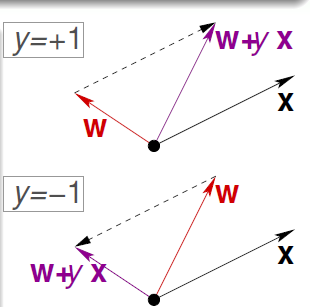
\includegraphics[width=5cm, height=5cm]{lecture2_2}\\
PLA \par
\end{center}
PLA Fact: $W_t$ Gets more Aligned with $W_f$,学习是能够保证$W$逐渐趋近于理想的$W_f$,
内积越大越相似。\par
\begin{align*}
w_f^{T}w_{t+1} &= w_f^{T}(w_t + y_{n(t)}x_{n(t)}) \\
               &\geq w_f^{T}w_t + \underset{n}{\min}y_nw_f^Tx_n \\
               &> w_f^Tw_t + 0.
\end{align*}
因此整个更新过程是$w_f \gets w_t$的,但有时候数据是有噪音的或者本身就不可分。 \par
% section section_name (end)
\begin{center}
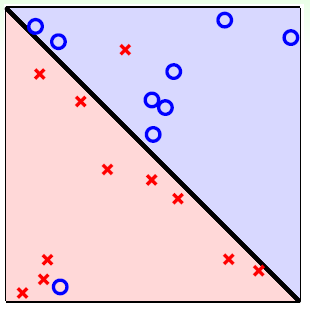
\includegraphics[width=5cm, height=5cm]{lecture2_3}\\
\end{center}
\subsection{Pocket}
\begin{algorithm}  
\caption{Pocket Algorithm}  
\begin{algorithmic}  
\STATE initialize pocket weights $\hat{w}$
\FOR{$t\gets1$ to $m$ }  
	\STATE 1.Find a \textcolor{Mycolor1}{mistake} of $W_t$
	\STATE eg. $sign(W_{t}^{T}x_{n(t)}) \neq y_{n(t)}$ 
	\STATE 2.$W_{t+1} \gets W_{t} + y_{n(t)}x_{n(t)}$ 
	\STATE 3.$W_{t+1} \gets \arg\underset{mistakes}{\min}(\hat{w},w_t)$
\ENDFOR
% \STATE return $W$(called W_{PLA})
\end{algorithmic}  
\end{algorithm}
\par
%%%%%%%%%%%%%%%%%%%%%Method one
\begin{bclogo}{Important!}
对PLA算法一个简单的修改(Pocket里永远是最好的),能处理有少许噪音的数据,但是速度要慢一点因为有比较的过程。 \par
\end{bclogo}
%%%%%%%%%%%%%%%%%%%%%Method tow
\begin{myremark}{Importance}
对PLA算法一个简单的修改(Pocket里永远是最好的),能处理有少许噪音的数据,但是速度要慢一点因为有比较的过程。 \par
\end{myremark}

\begin{center}
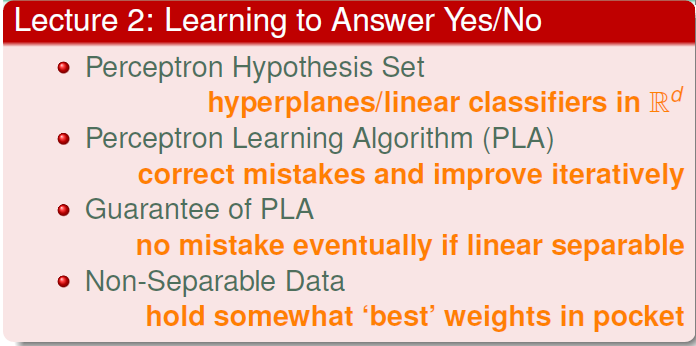
\includegraphics[width=10cm, height=5.5cm]{lecture2_sum}\\
\end{center}

\noindent
{\color{RubineRed} \rule{\linewidth}{1mm} }